\chapter{Line Segment Tracking}\label{ch:lst}

\section{The HL-LHC computing challenge}
With the massive increase in pileup in the HL-LHC era, each recorded event is massively more complex, making all steps of data processing much more expensive. 
Current projects show that, in fact, computing demands will exceed the resources that CMS is able to provide, even with annual increases (Fig.~\ref{fig:cpu_curve}). 
We must therefore make use of novel hardware or develop more efficient algorithms to make HL-LHC operations at all possible at CMS. 
In particular, reconstruction will represent 61\% of CPU usage at CMS when the HL-LHC turns on (Fig.~\ref{fig:cpu_pie}), and a large fraction of that compute is dedicated to track reconstruction. 

\begin{figure}[htb]
    \centering
    \subfloat[]{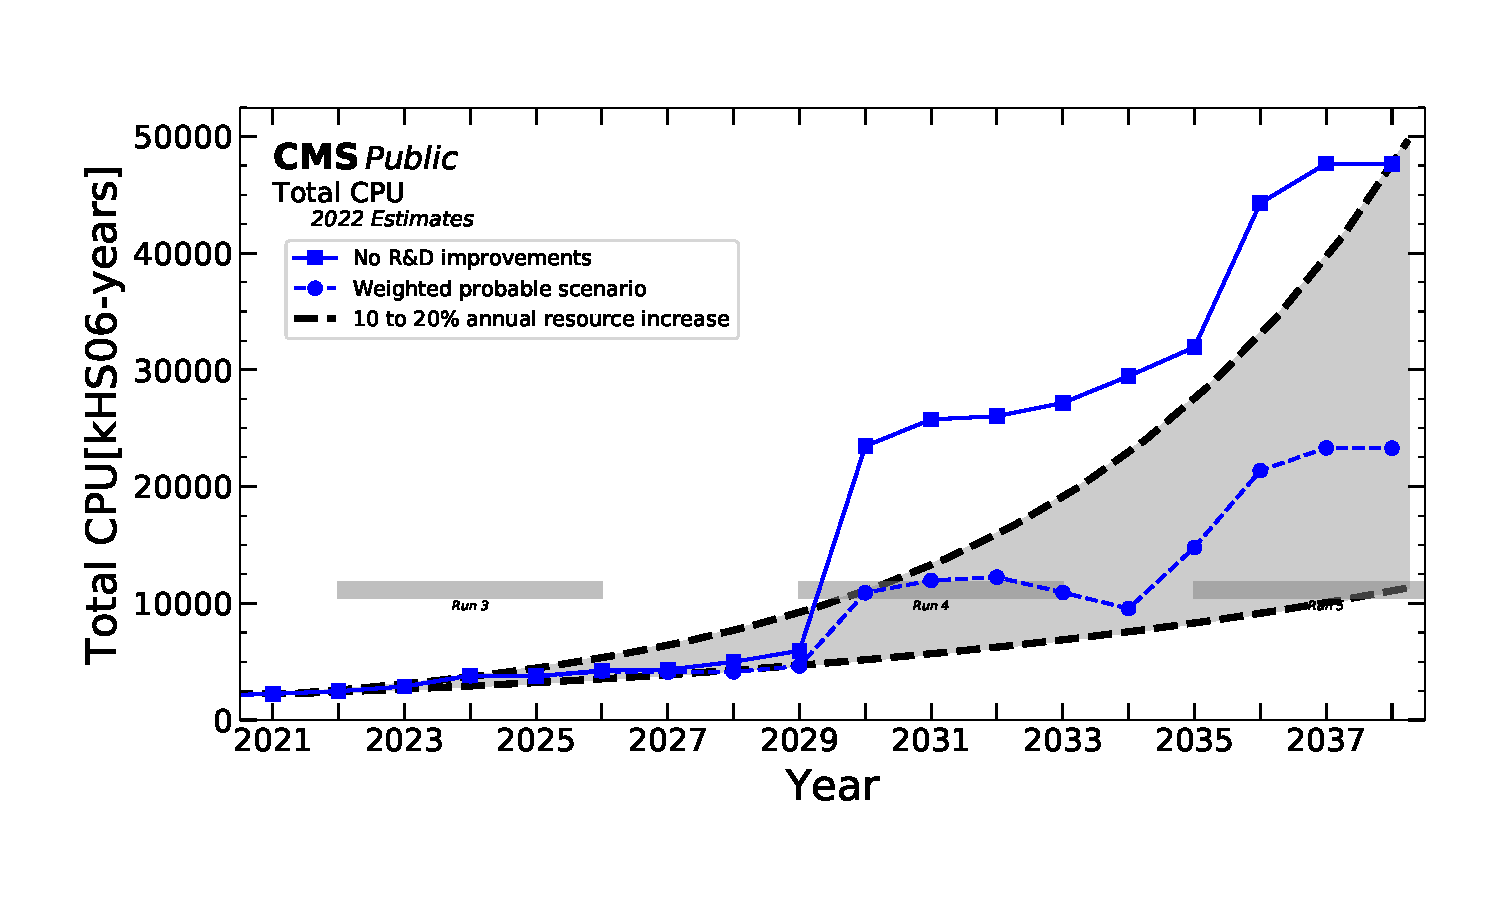
\includegraphics[width=0.55\linewidth,valign=c]{fig/lst/cpu_cms2022.pdf}\label{fig:cpu_curve}}
    % No \qquad needed because there is so much whitespace in these PDFs
    \subfloat[]{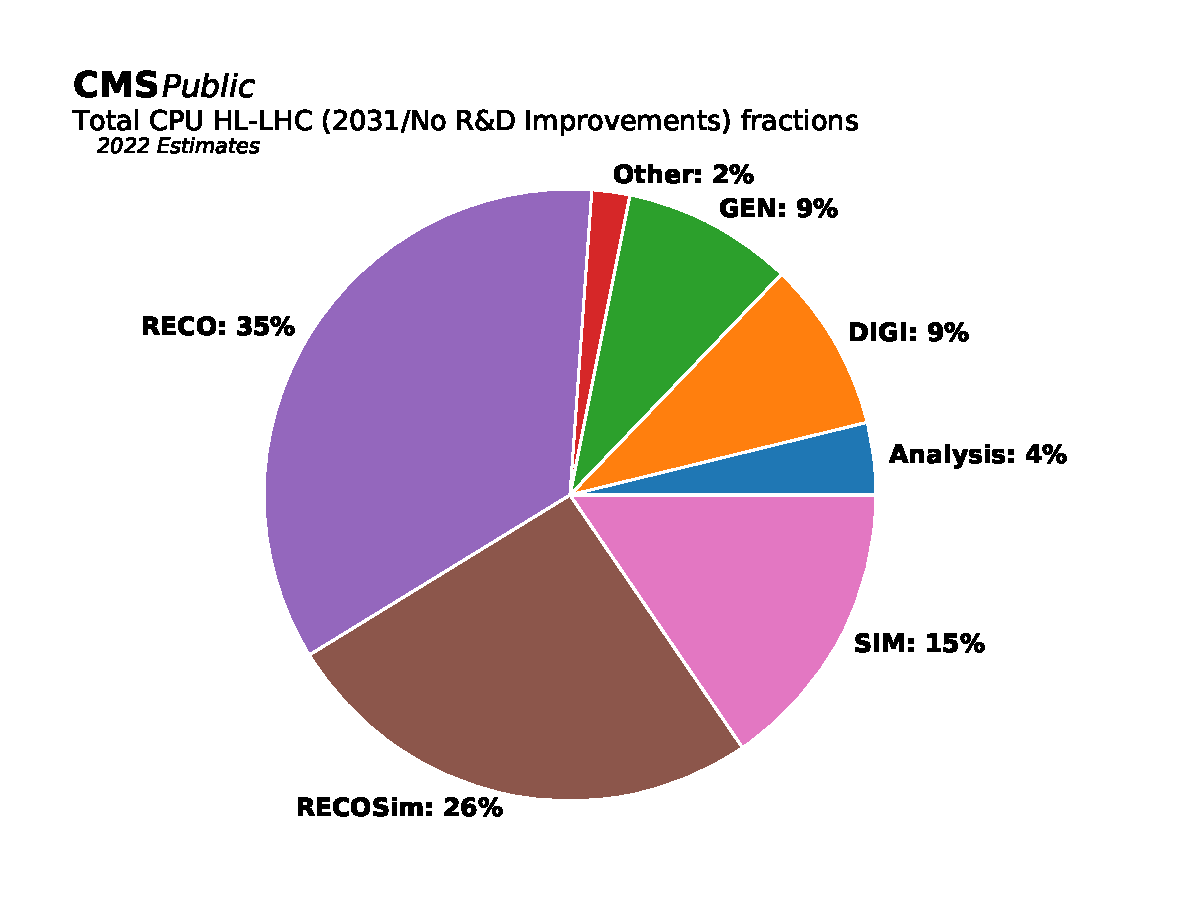
\includegraphics[width=0.4\linewidth,valign=c]{fig/lst/cpu_pie_cms2022.pdf}\label{fig:cpu_pie}}
    \caption[HL-LHC CPU usage projections at CMS]{
        The HL-LHC CPU usage projections at CMS as a function of time (left) and broken down by computing tasks (right), from Ref.~\cite{CMSComputingReport2022}. 
    }
    \label{fig:cpu_projections}
\end{figure}

\subsection{Track reconstruction}
Because many thousands of particles are produced simultaneously in each bunch crossing, individual tracks need to be recognized out of dense clouds of x-y-z points called ``hits'' (Fig.~\ref{fig:tracking_cartoon}).
This is made even more challenging with the HL-LHC, where tens of pileup collisions becomes hundreds.
Nevertheless, individual particle tracks \textit{must} be reconstructed because they contain critical information about what was produced in the collision.
This is accomplished in two steps: track finding and track fitting.
First, a track-finding algorithm identifies each set of hits that were likely to have been generated by the same particle---these are called track ``candidates.''
Then, a track-fitting algorithm takes each track candidate and fits a trajectory to it, from which it can determine key properties of the particle like its charge and momentum.

\begin{figure}[!htb]
    \centering
    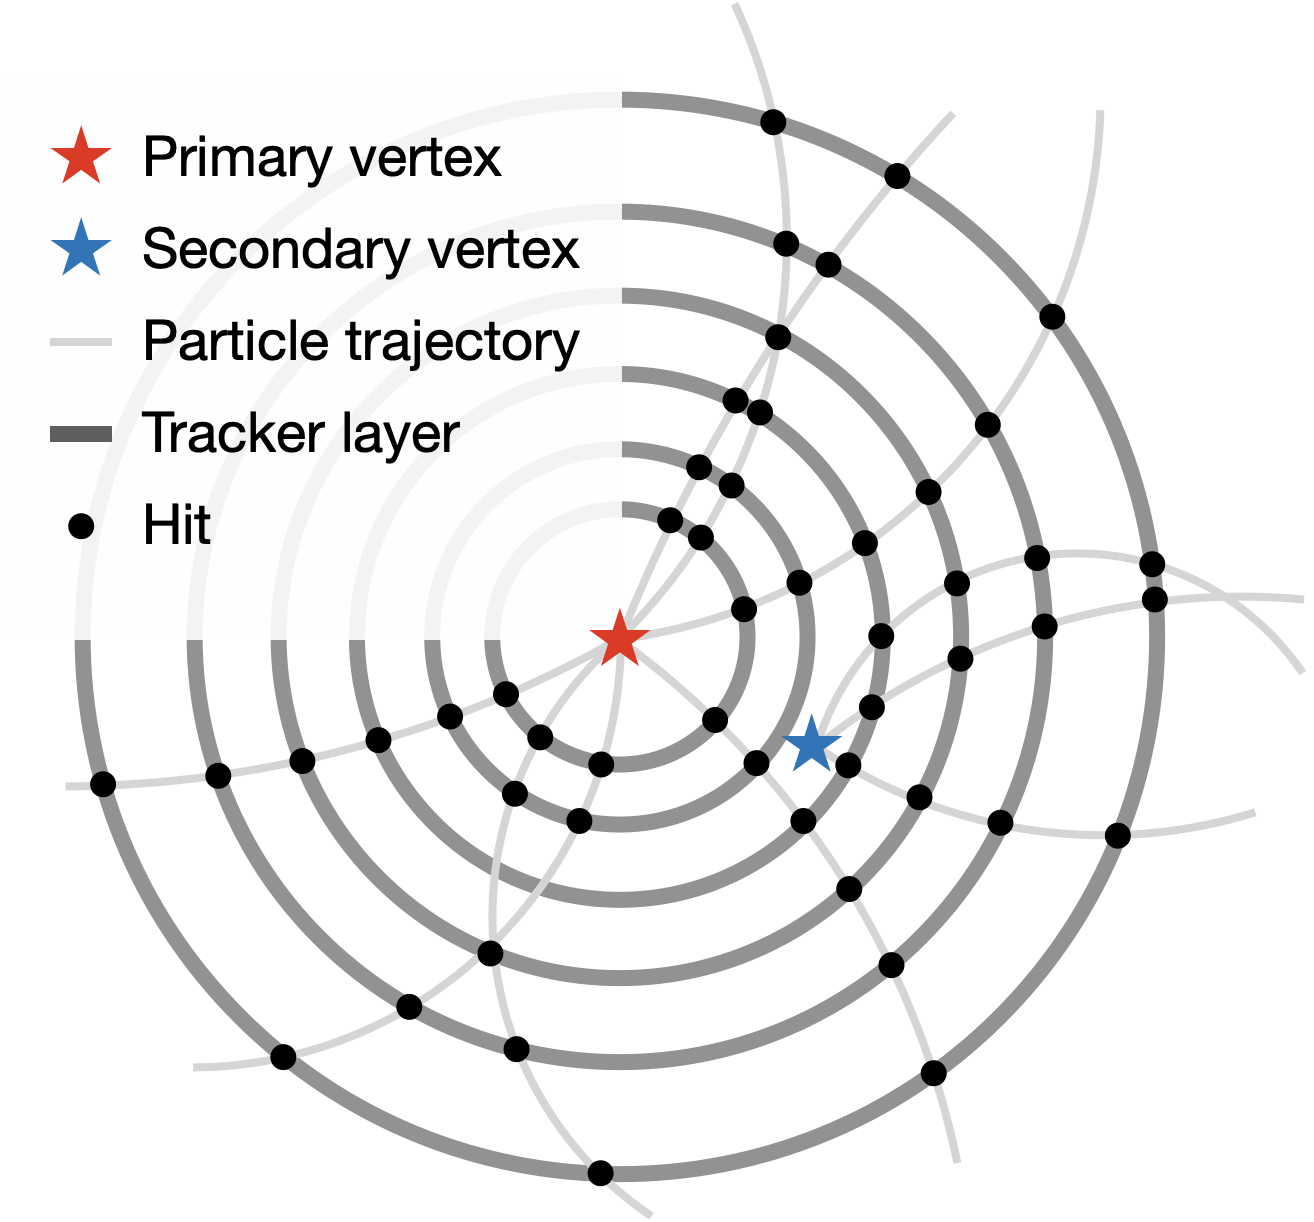
\includegraphics[width=0.45\linewidth]{fig/lst/tracking_cartoon.png}
    \caption[Simple illustration of particles leaving hits in a multi-layered tracker]{
        Simple illustration of particles (grey lines) leaving hits (black dots) in a multi-layered tracker. 
    }
    \label{fig:tracking_cartoon}
\end{figure}

Better track-fitting yields more accurate ``track parameters'' that are crucial for downstream analysis. 
For example, those same algorithms that use the presence of displaced tracks to identify longer-lived particles rely on the accuracy of the input features. 
While not a central topic of this chapter, there is already a well-optimized solution for track-fitting~\cite{cerati2023generalizing}.

Better track-finding yields a higher quantity and quality of reconstructed tracks, enabling more diverse and precise analysis.
Moreover, many interesting physics processes involve particles that decay in flight after traveling millimeters to centimeters (and beyond in some cases), resulting in ``displaced'' tracks that do not point to a proton-proton collision.
The Higgs boson, a primary object of interest, can only be detected by identifying its decay products, some of which have longer lifetimes~\cite{Bols:2020bkb}. 
Many new physics candidates are also expected to have long lifetimes (e.g. Ref.~\cite{CMS:2023bay}), so it is imperative that track-finding algorithms are robust against edge cases---in addition to displaced production vertices, tracks can also have holes or significant overlap.
Finally, with the massive increase in pileup, track finding also becomes a problem of computational scalability, adding yet another dimension to the problem of track finding: proposed algorithms must meet or exceed critical efficiency milestones while being robust to vital edge cases and delivering massive gains in throughput all at once.

Traditional track-finding algorithms, namely the Kalman filter, proceed sequentially, building tracks from the innermost to the outermost layer of the silicon tracker. 
Moreover, this means that track-finding at CMS is currently completely reliant on the pixel detector, which is more prone to failures due to its proximity to the beamline, and displaced tracks that begin in the outer tracker are more easily missed.

\section{The line segment tracking algorithm}
Proposed originally as a drastic redesign of the silicon tracker layers, the line segment tracking (LST) algorithm makes use of the bi-layer ``\pt-modules'' that will replace the single-layer tracking modules currently used in the outer tracker. 
Each of these modules will have two silicon sensors spaced a few millimeters apart~\cite{CERN-LHCC-2017-009}, allowing for a rough estimation of a throughgoing particle's \pt (Fig.~\ref{fig:ph2_tracker}). 
That is, particles with high-\pt will have two hits within a small window, so particles with two hits outside of that window have low-\pt and can most likely be rejected. 
This massively reduces the occupancy (number of hits) in the tracker due to pileup, which produces mostly low-\pt particles. 

\begin{figure}[!htb]
    \centering
    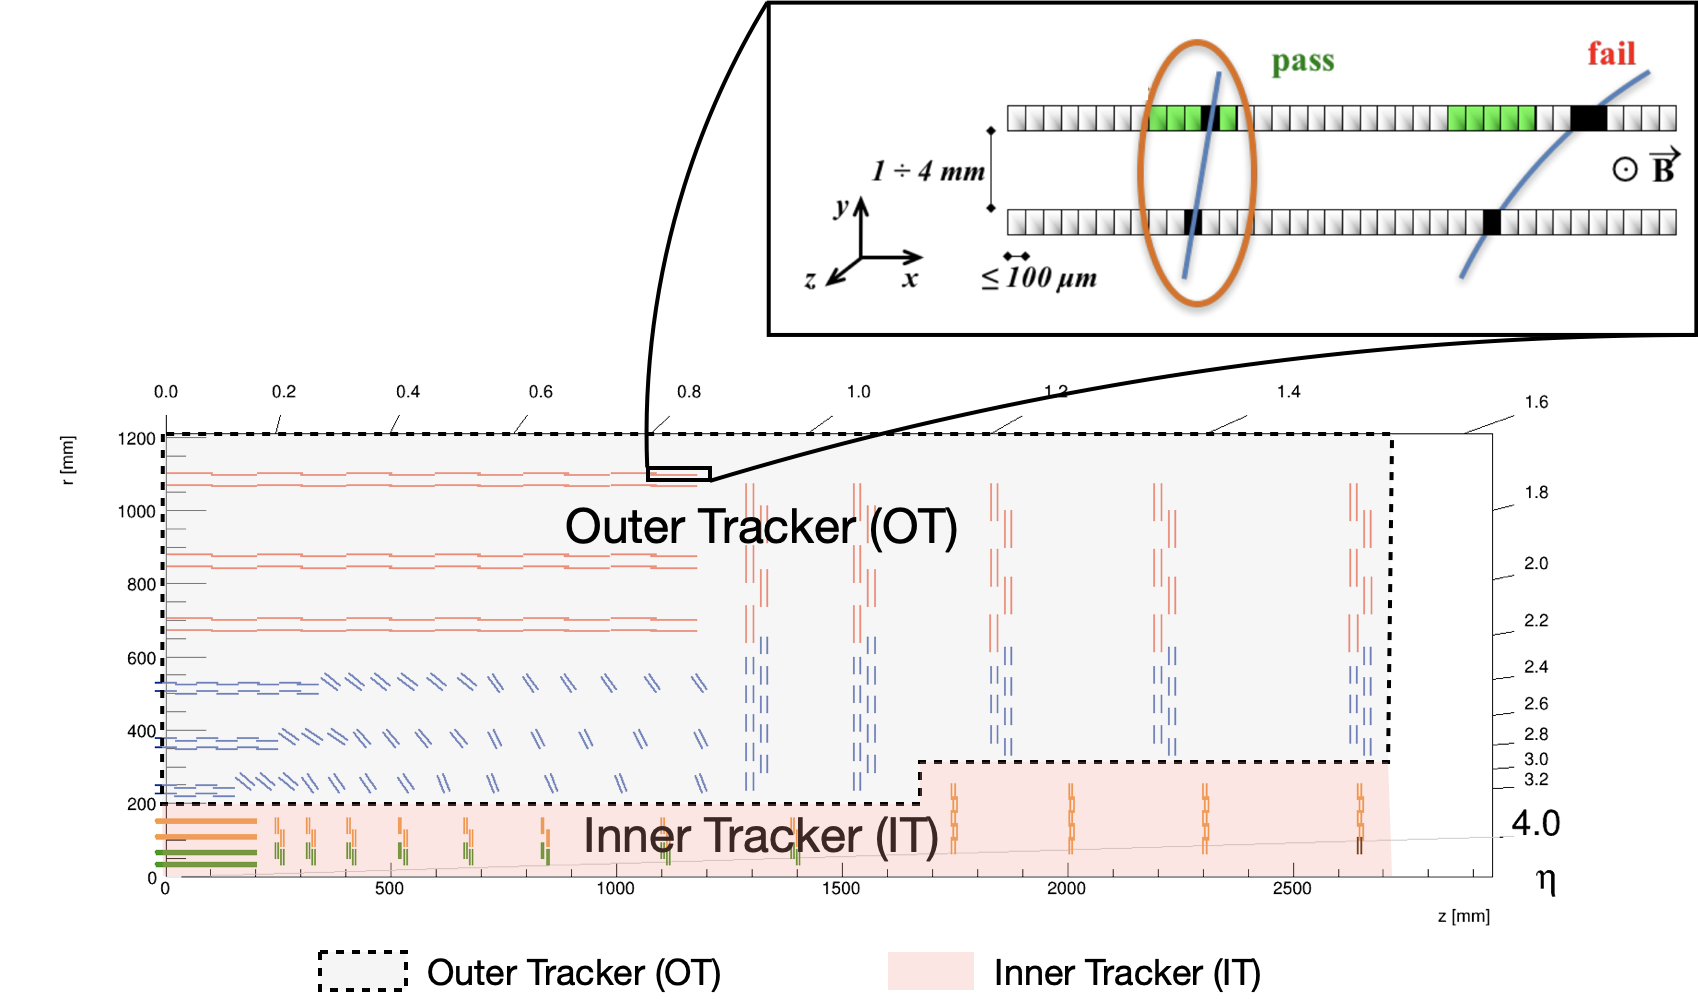
\includegraphics[width=0.75\linewidth]{fig/lst/tracker_with_pt_module.png}
    \caption{
        An illustration of the CMS Phase-II silicon tracker with a diagram of a \pt-module from Ref.~\cite{CMS-DP-2023-075}. 
    }
    \label{fig:ph2_tracker}
\end{figure}

Rather than build every track hit-by-hit, LST builds track segments of increasing size in parallel, leveraging GPUs for a massive speedup. 
Starting in the outer tracker, LST first builds ``mini-doublets'' (MDs) in each \pt-module, filtering out low-\pt tracks. 
Then, line segments (LSs) are built from each pair of MDs in  adjacent tracker layers, and each LS is required to contain MDs with consistent \pt estimates. 
Progressively longer track segments are built in this way: ``triplets'' (T3s) are formed from LSs that share a MD, and ``quintuplets'' (T5s) are formed from T3s that share a MD. 
At each step, the track segments are required to be approximately consistent with a single helical trajectory. 
Finally, the track segments in the pixel layer (pLSs) are taken from an upstream algorithm and matched to the LST track segments, resulting in four mutually exclusive collections of track candidates (TCs). 
First, pLSs are matched to T5s, forming pT5s. 
Next, the unmatched T5s are set aside, and the T3s that are not in a pT5 are matched to pLSs, forming pT3s. 
Last, all unused pLSs are collected and considered also as track candidates. 
A complete taxonomy of the LST objects, along with a summary of the steps detailed here, is presented in Table~\ref{tab:lst}.

\begin{table}[htb]
    \centering
    \caption[LST track-finding steps and object definitions]{
        The steps of the LST algorithm are shown in order of execution, starting with track-segment building (Steps 1 to 4) followed by track-candidate selection (Steps 5 to 8).
        Step 0 is performed by a preceding iteration of the CMS track-finding algorithm.
        Each LST step is implemented as a separate kernel, where the track objects of interest are built in parallel.
    }
    \label{tab:lst}
    \begin{tabular}{ccp{10cm}}
        \toprule
        Step & Track segment       & Description                              \\
        \midrule
        0 & Pixel seeds (pLSs)  & Track segments from the inner tracker       \\
        1 & Mini-doublets (MDs) & Two hits in a \pt-module                    \\
        2 & Line segments (LSs) & Two MDs in nearby modules                   \\
        3 & Triplets (T3s)      & Two LSs that share a common MD              \\
        4 & Quintuplets (T5s)   & Two T3s that share a common MD              \\
        \toprule
        Step & Track candidate     & Description                              \\
        \midrule
        5 & pT5s & T5s matched to a pixel seed                                \\
        6 & T5s  & T5s that are not matched to a pixel seed                   \\
        7 & pT3s & T3s that are not in a pT5, but are matched to a pixel seed \\
        8 & pLS  & Pixel seeds that are not already in a pT5 or pT3           \\
        \bottomrule
    \end{tabular}
\end{table}

We benchmark LST with a variety of MC simulation samples. 
Primarily, we use simulated \ttbar events, which have displaced tracks (from \PQb quarks) and multiple jets, and therefore a high tracker occupancy, with a pileup of 200 (PU200) and the Phase-II tracker geometry. 
In order to measure the performance of LST, we look at each simulated track and try to match it to a TC: if more than 75\% of the hits in a TC belong to a single simulated track, it is considered as real. 
Then, the efficiency is defined as the fraction of simulated tracks that are matched in this way to a TC, whereas the fake rate is defined as the fraction of TCs that are not matched to any simulated tracks. 
These two metrics are plotted in Fig.~\ref{fig:lst_performance}, where it is clear that the fake TCs in the barrel are mostly T5s, which also contribute the largest fraction of the overall efficiency. 
In the baseline version of LST, there is therefore an opportunity for massive improvement. 

\begin{figure}[!htb]
    \centering
    \subfloat{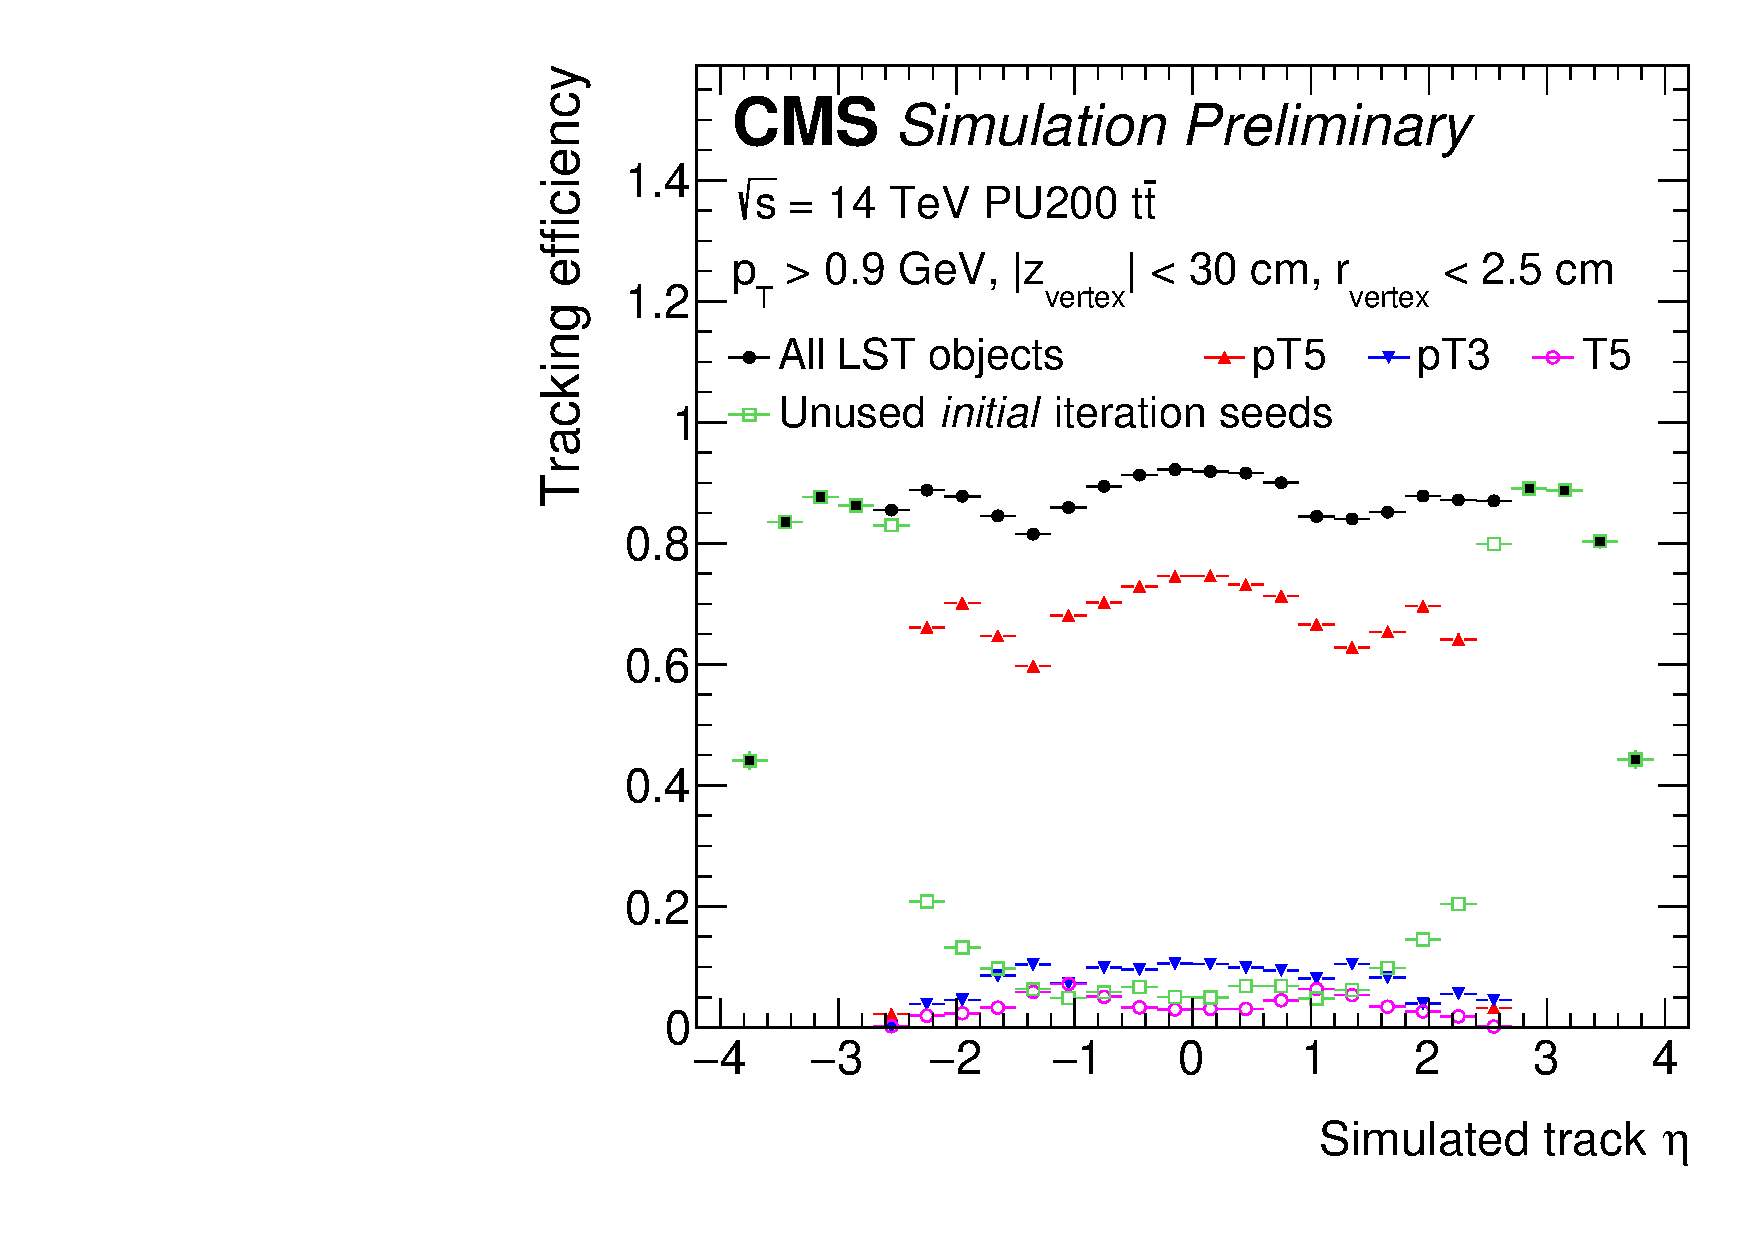
\includegraphics[width=0.45\linewidth]{fig/lst/standalone_Master_eff_etacourse.pdf}}
    \qquad
    \subfloat{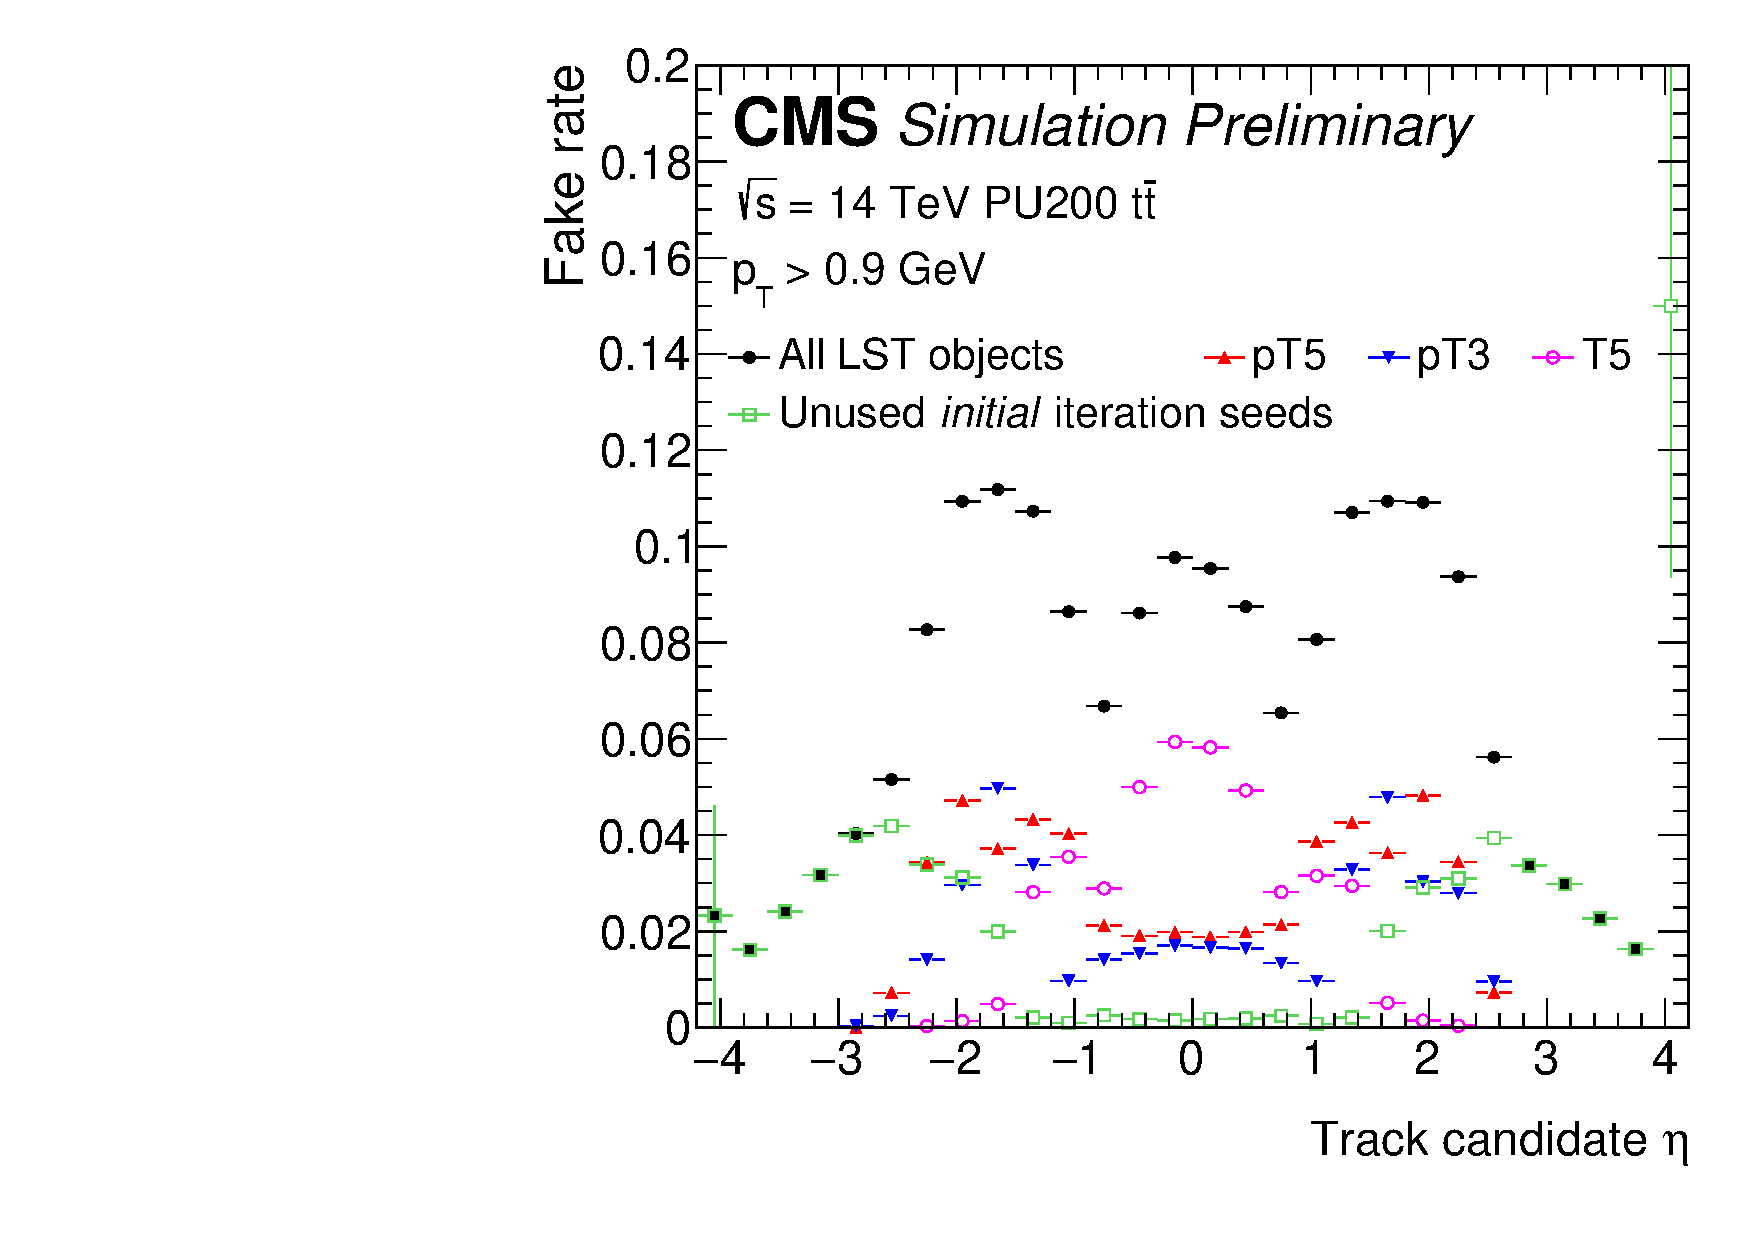
\includegraphics[width=0.45\linewidth]{fig/lst/standalone_Master_fr_etacourse.pdf}}
    \caption[LST track-finding efficiency and fake rate plotted as a function of $\eta$]{
        The LST track-finding efficiency (left) and fake rate (right) plotted as a function of the pseudorapidity $\eta$ of the simulated track and track candidate respectively.
        For both plots, five histograms are overlaid: all track candidates (black), pT5s (red), pT3s (blue), T5s (magenta), and pLSs that are not used in a pT5 or pT3 (green).
        On the left, it can be seen that T5s comprise the majority of the LST track-finding efficiency, either as pT5s or T5s.
        On the right, it can also be seen that the T5s make up the bulk of the LST fake rate in the barrel region.
    }
    \label{fig:lst_performance}
\end{figure}

\section{Improving LST with machine learning}

\subsection{Training}
We trained a DNN on the set of T5s built by LST running on 175 \ttbar PU200 events with the selections on a custom heuristic on the quality of a circular fit to the T5 in the $r$-$\phi$ plane removed under the assumption that the DNN could better use the same information. 
In total, this yielded approximately 840\,000 real T5s and 1.26 million fake T5s shuffled into two datasets, 80\% for training and 20\% for testing. 

The DNN receives input features describing the orientation and \pt of each T3, the T5 itself, and the ``bridge T3'' that connects the three MDs at the center of the T5 (Fig.~\ref{fig:t5_anatomy}). 
The coordinates of the ``anchor'' hit in each MD are also provided---for PS \pt-modules, the hit in the P-layer is taken as the anchor hit, whereas the innermost hit is taken as the anchor hit for 2S modules. 
There are 38 input features in total: the \pt estimate and radius of a circular fit to the hits in each of the T3s; 
the $(r, \phi, z)$ coordinates, $\eta$, and layer of each anchor hit; 
the \pt estimate, $\eta$, and $\phi$ of the T5; 
and the radius of a circular fit to the hits in the bridge T3. 
Because the DNN will classify T5s as fake or real, binary cross entropy is used as the loss function. 

\begin{figure}[!htb]
    \centering
    \subfloat[]{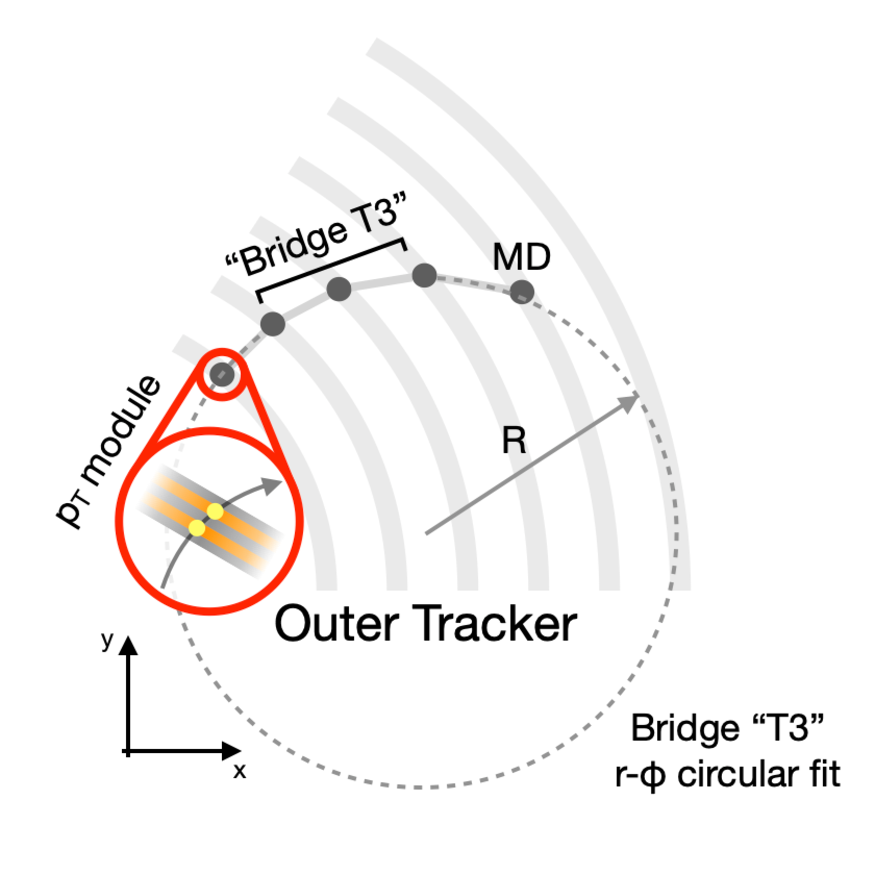
\includegraphics[width=0.35\linewidth]{fig/lst/T5_anatomy.pdf}\label{fig:t5_anatomy}}
    \qquad
    \subfloat[]{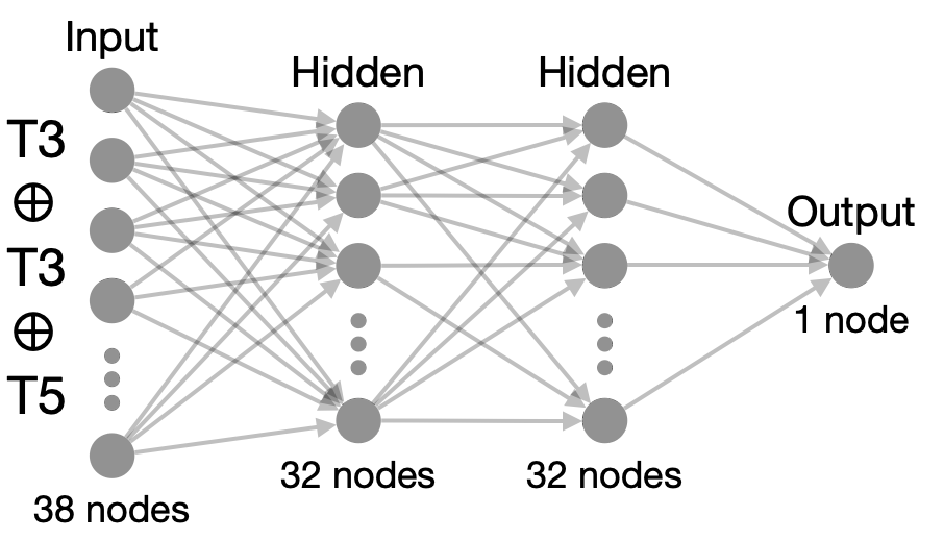
\includegraphics[width=0.55\linewidth]{fig/lst/T5_DNN_architecture.pdf}\label{fig:t5dnn_arch}}
    \caption[The components of a T5 and the DNN architecture]{
        The components of a T5 in the $r$-$\phi$ plane, including the ``bridge'' T3, the circular fit, and the anchor hit in a MD (left) alongside the DNN architecture used in this work (right). 
    }
\end{figure}

Given the relatively simple input, and the intense throughput requirements of LST, we selected a simple DNN architecture: a two-layer DNN with 32 nodes per hidden layer. 
The DNN was trained for over 600 epochs, but the loss plateaued after epoch 400 (Fig.~\ref{fig:t5dnn_history}). 
The ROC curve at epoch 500 is shown in Fig.~\ref{fig:t5dnn_roc}; larger architectures were explored, but we found that they did not give significantly better performance. 
Compared to LST, the DNN is able to reduce the number of false positives---fake T5s incorrectly classified as real---by nearly 50\%. 

\begin{figure}[!htb]
    \centering
    \subfloat[]{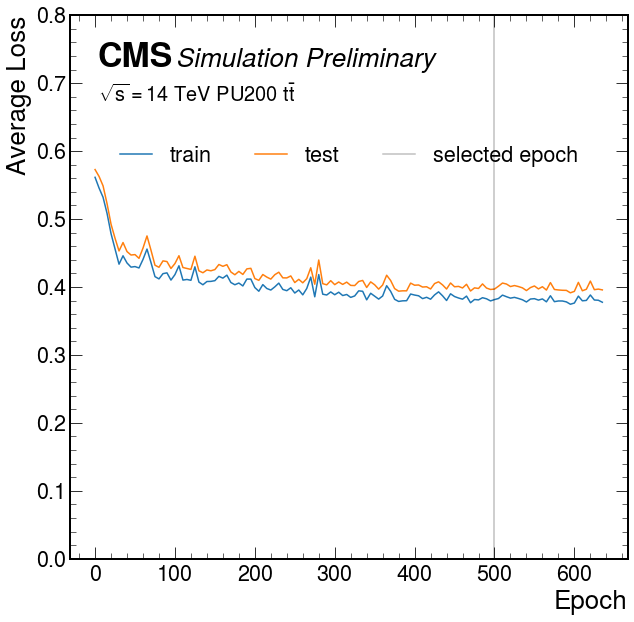
\includegraphics[width=0.45\linewidth]{fig/lst/main_history.png}\label{fig:t5dnn_history}}
    \qquad
    \subfloat[]{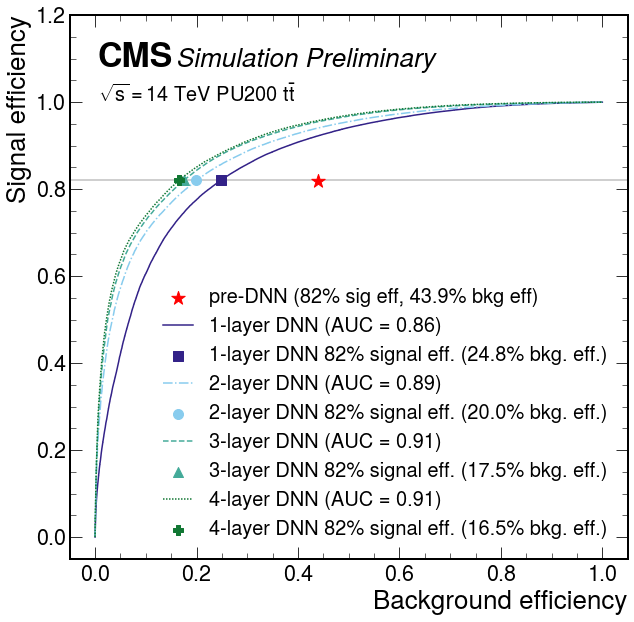
\includegraphics[width=0.45\linewidth]{fig/lst/roc.png}\label{fig:t5dnn_roc}}
    \caption[The average loss after each epoch and ROC curve for the DNN]{
        The average loss after each epoch plotted (a) next to the Receiver Operating Characteristic (ROC) curves for the model after epoch 500 (b). 
        For the ROC curve, the signal efficiency is plotted on the y-axis, while the background efficiency, or fake rate, is plotted on the x-axis. 
    }
\end{figure}

\subsection{Results}
After verifying that the DNN could classify T5s better than the cuts removed from LST, it was integrated into the LST algorithm so the effect on the final collection of TCs could be evaluated. 
A working point for the DNN was selected to match the baseline LST true positive rate---the number of T5s correctly classified as real. 
As such, no loss of efficiency is observed with the DNN integrated into the algorithm (Fig.~\ref{fig:t5dnn_eff}). 
However, the efficiency binned in the displacement of the track tells a different story (Fig.~\ref{fig:t5dnn_dis}): the DNN recovers displaced tracks that were being dropped by LST. 
Meanwhile, the fake rate (Fig.~\ref{fig:t5dnn_fkr}) is reduced by 40\% on average in the barrel, addressing the motivation for this work. 
These performance enhancements come at no cost in throughput (Fig.~\ref{fig:streams-vs-throughput}).

\begin{figure}[!htb]
    \centering
    \subfloat{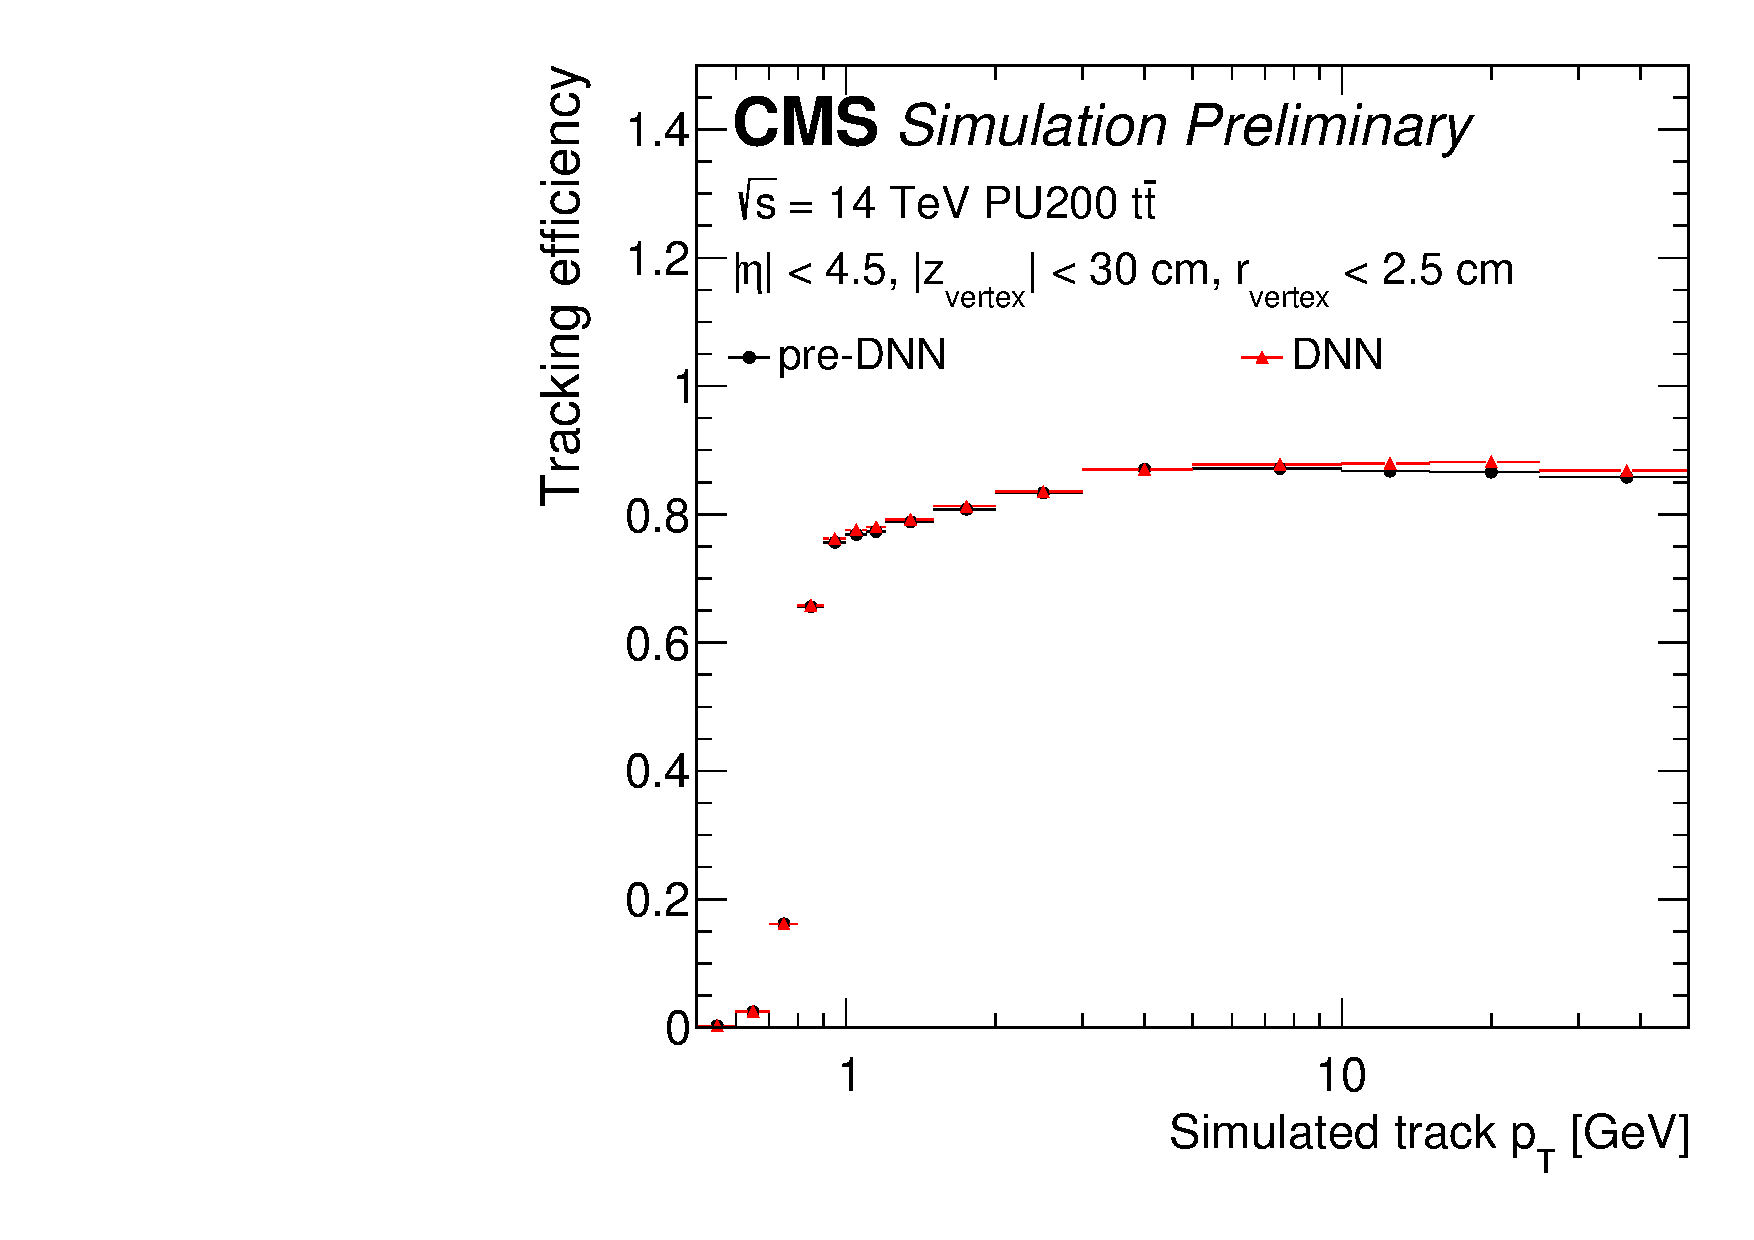
\includegraphics[width=0.45\linewidth]{fig/lst/standalone_DNNvsMaster_pu200_eff_pt_logx.pdf}}
    \qquad
    \subfloat{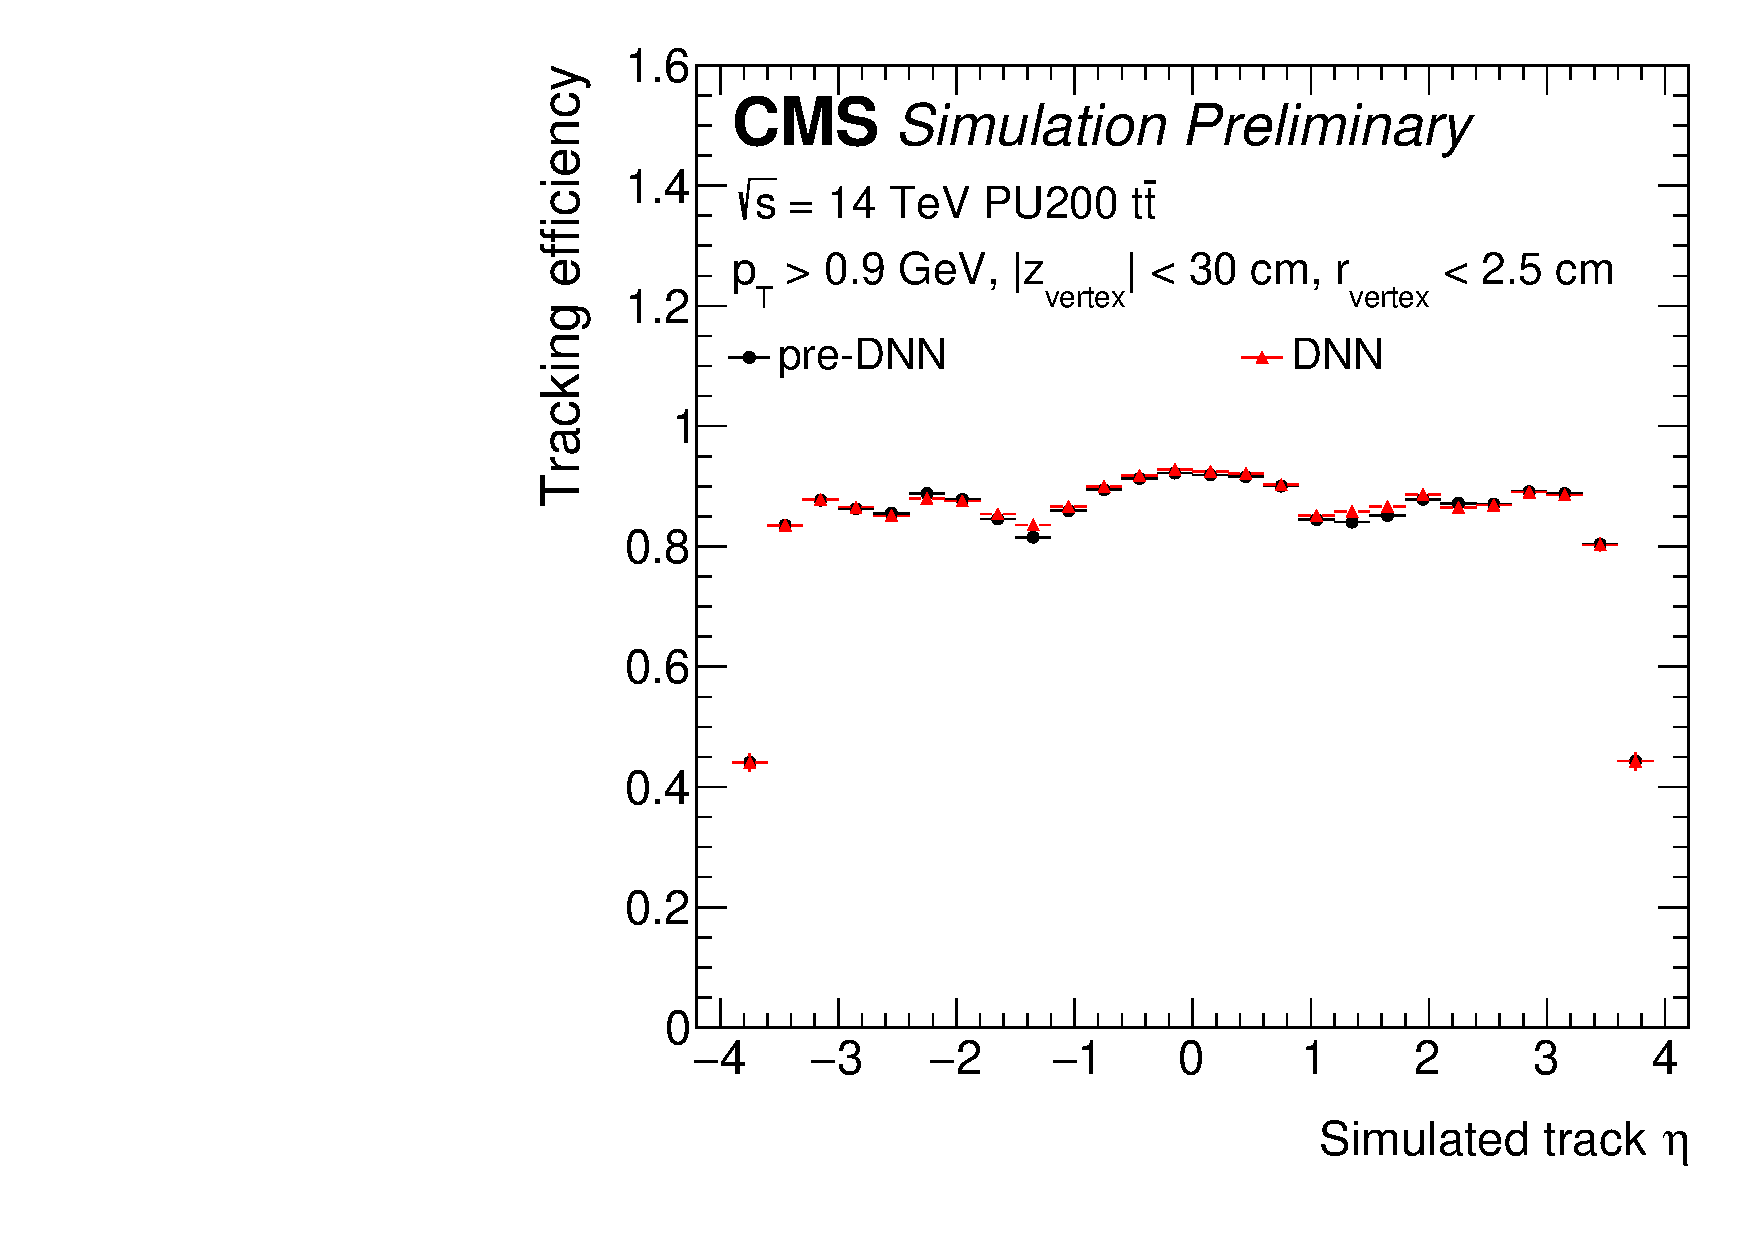
\includegraphics[width=0.45\linewidth]{fig/lst/standalone_DNNvsMaster_pu200_eff_etacourse.pdf}}
    \caption[LST efficiency for all TCs plotted as a function of \pt and $\eta$]{
        The LST efficiency for all TCs plotted as a function of \pt (left) and $\eta$ (right).
        The working point for the DNN was selected to match the efficiency of LST, and it is clear that no efficiency is lost.
    }
    \label{fig:t5dnn_eff}
\end{figure}

\begin{figure}[!htb]
    \centering
    \subfloat{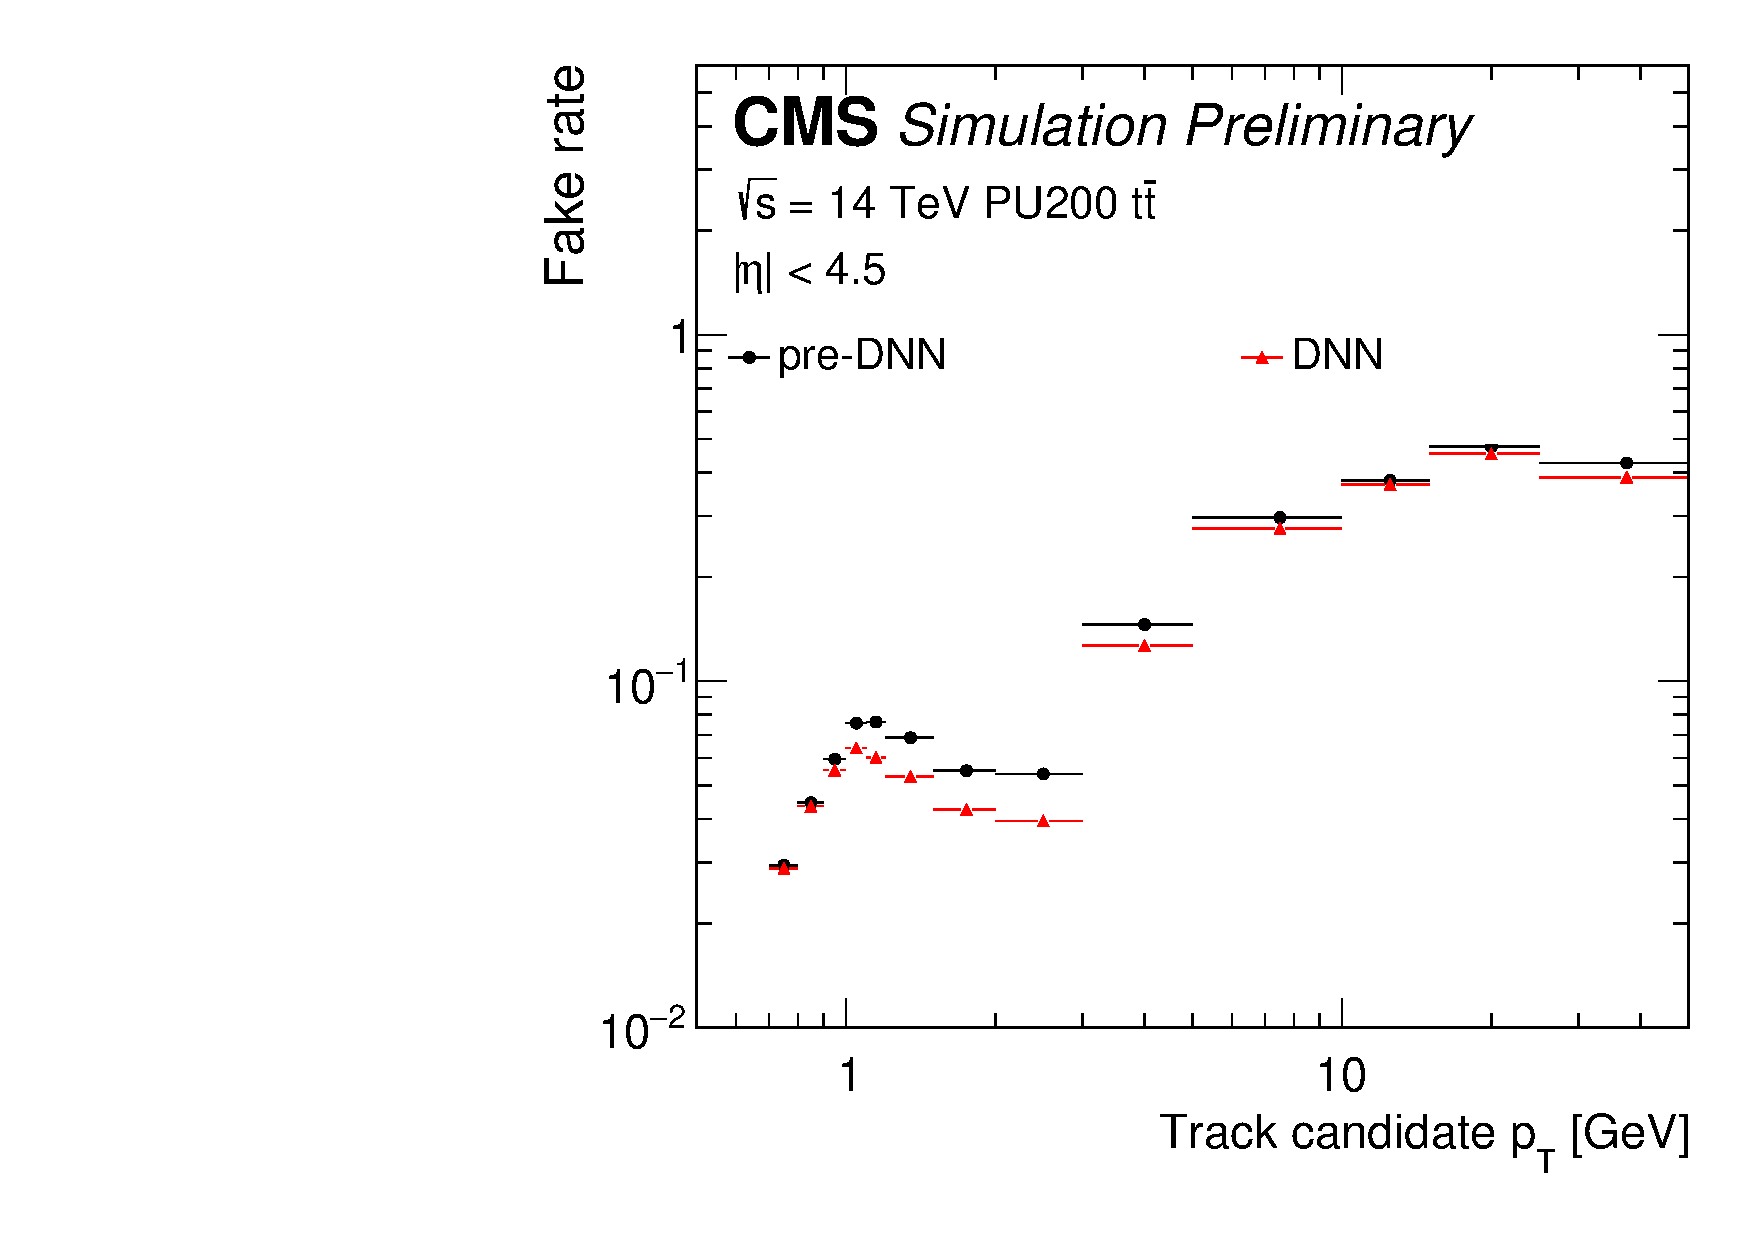
\includegraphics[width=0.45\linewidth]{fig/lst/standalone_DNNvsMaster_pu200_fr_pt_logx_logy.pdf}}
    \qquad
    \subfloat{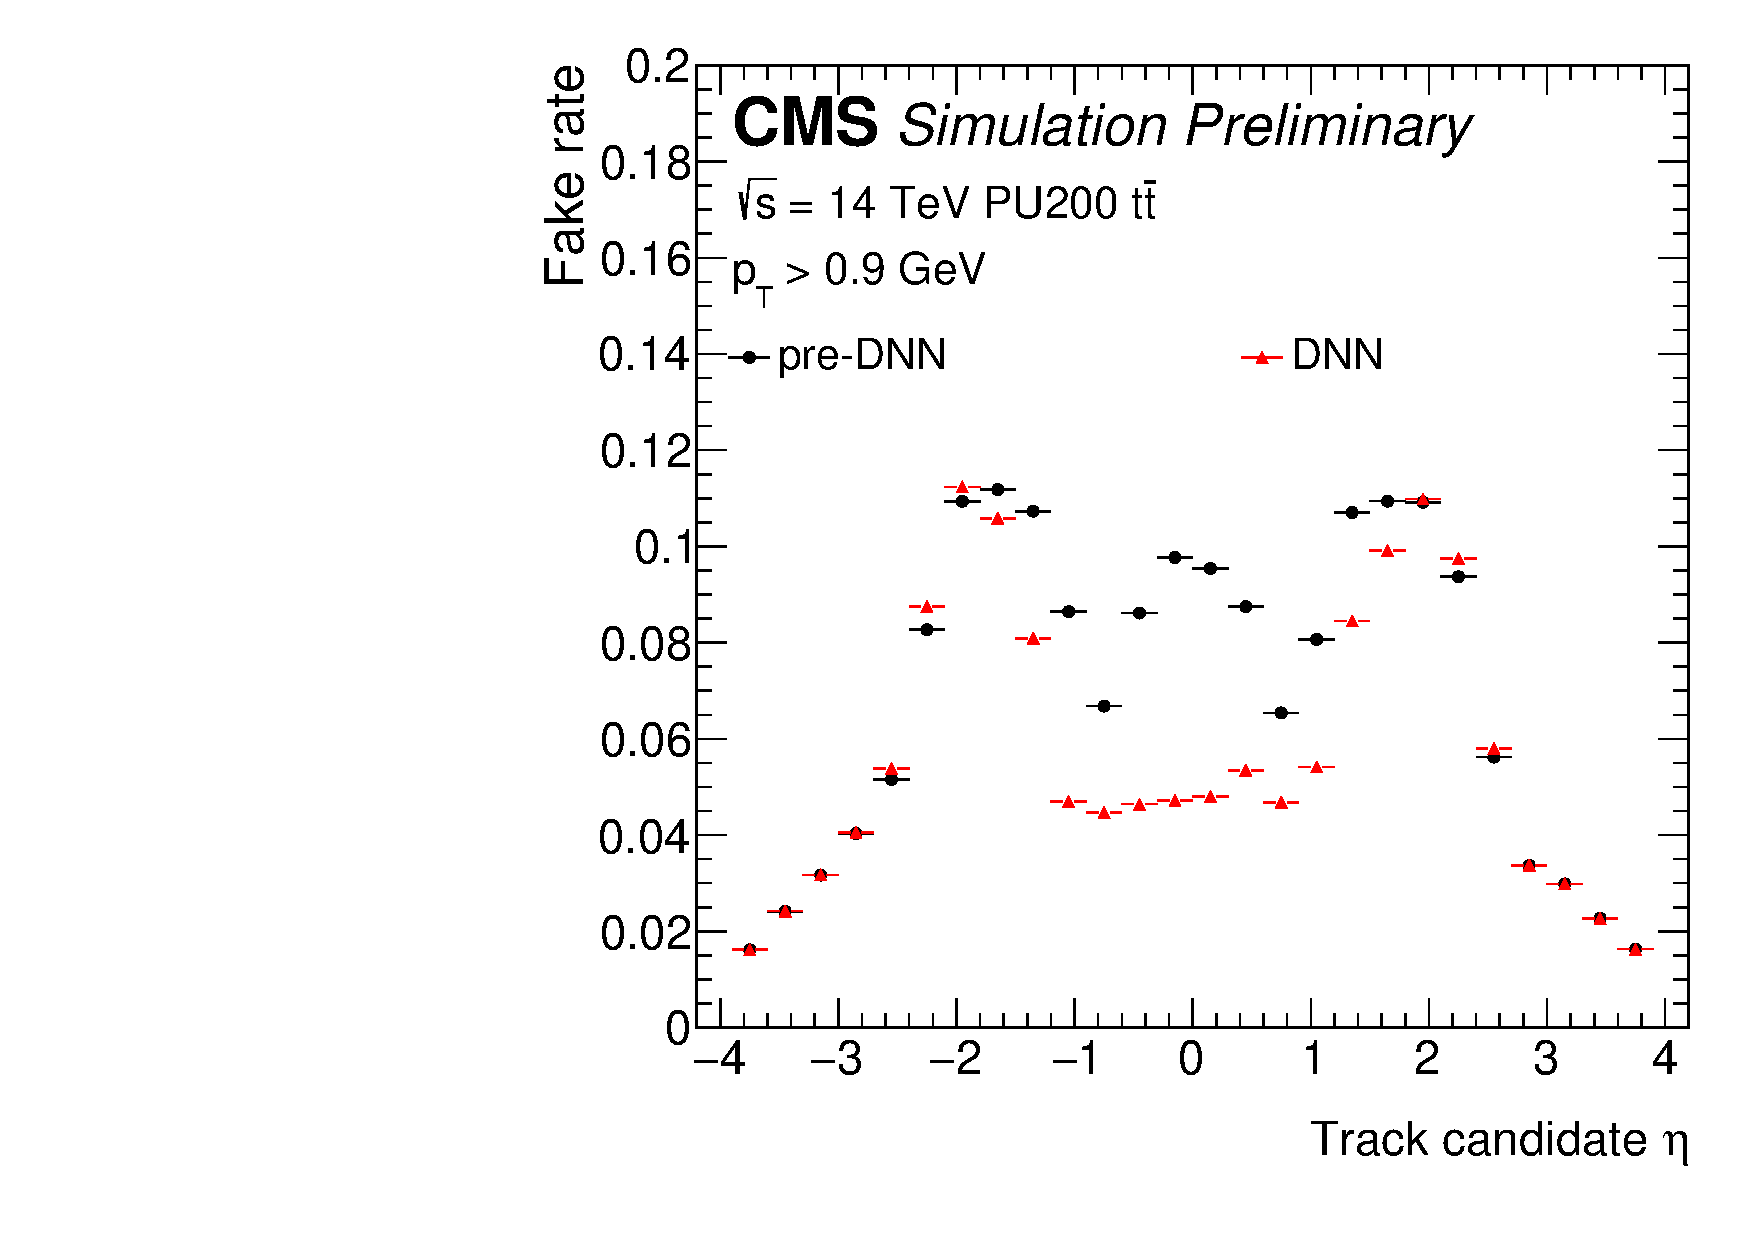
\includegraphics[width=0.45\linewidth]{fig/lst/standalone_DNNvsMaster_pu200_fr_etacourse.pdf}}
    \caption[LST fake rate for all TCs plotted as a function of \pt and $\eta$]{
        The LST fake rate for all TCs plotted as a function of \pt (left) and $\eta$ (right).
        Notably, there is a 40\% reduction in the fake rate in the barrel, where the T5 fake rate was previously dominant.
    }
  \label{fig:t5dnn_fkr}
\end{figure}

\begin{figure}[!htb]
    \centering
    \subfloat[]{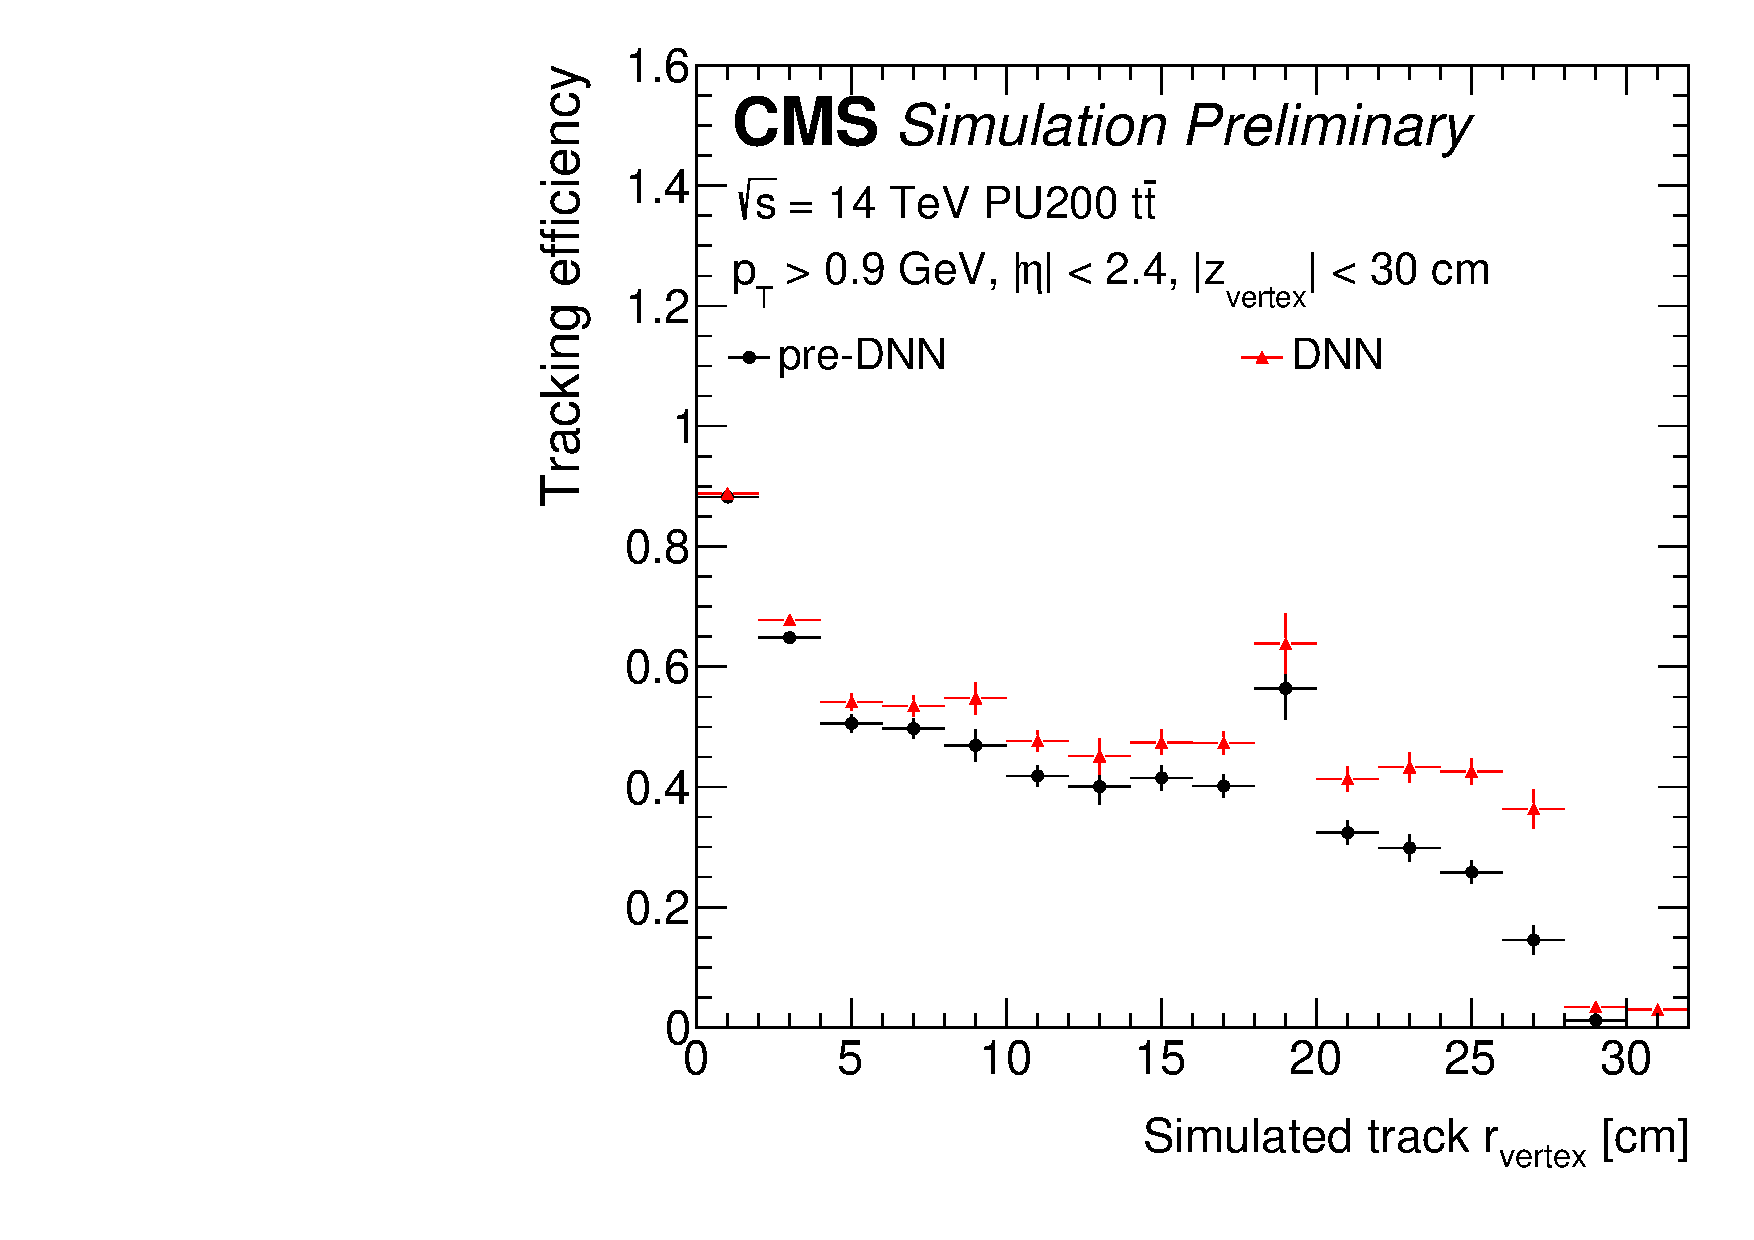
\includegraphics[width=0.45\linewidth]{fig/lst/standalone_DNNvsMaster_pu200_loweta_eff_vxycoarse.pdf}\label{fig:t5dnn_eff_rvertex_ttbar}}
    \qquad
    \subfloat[]{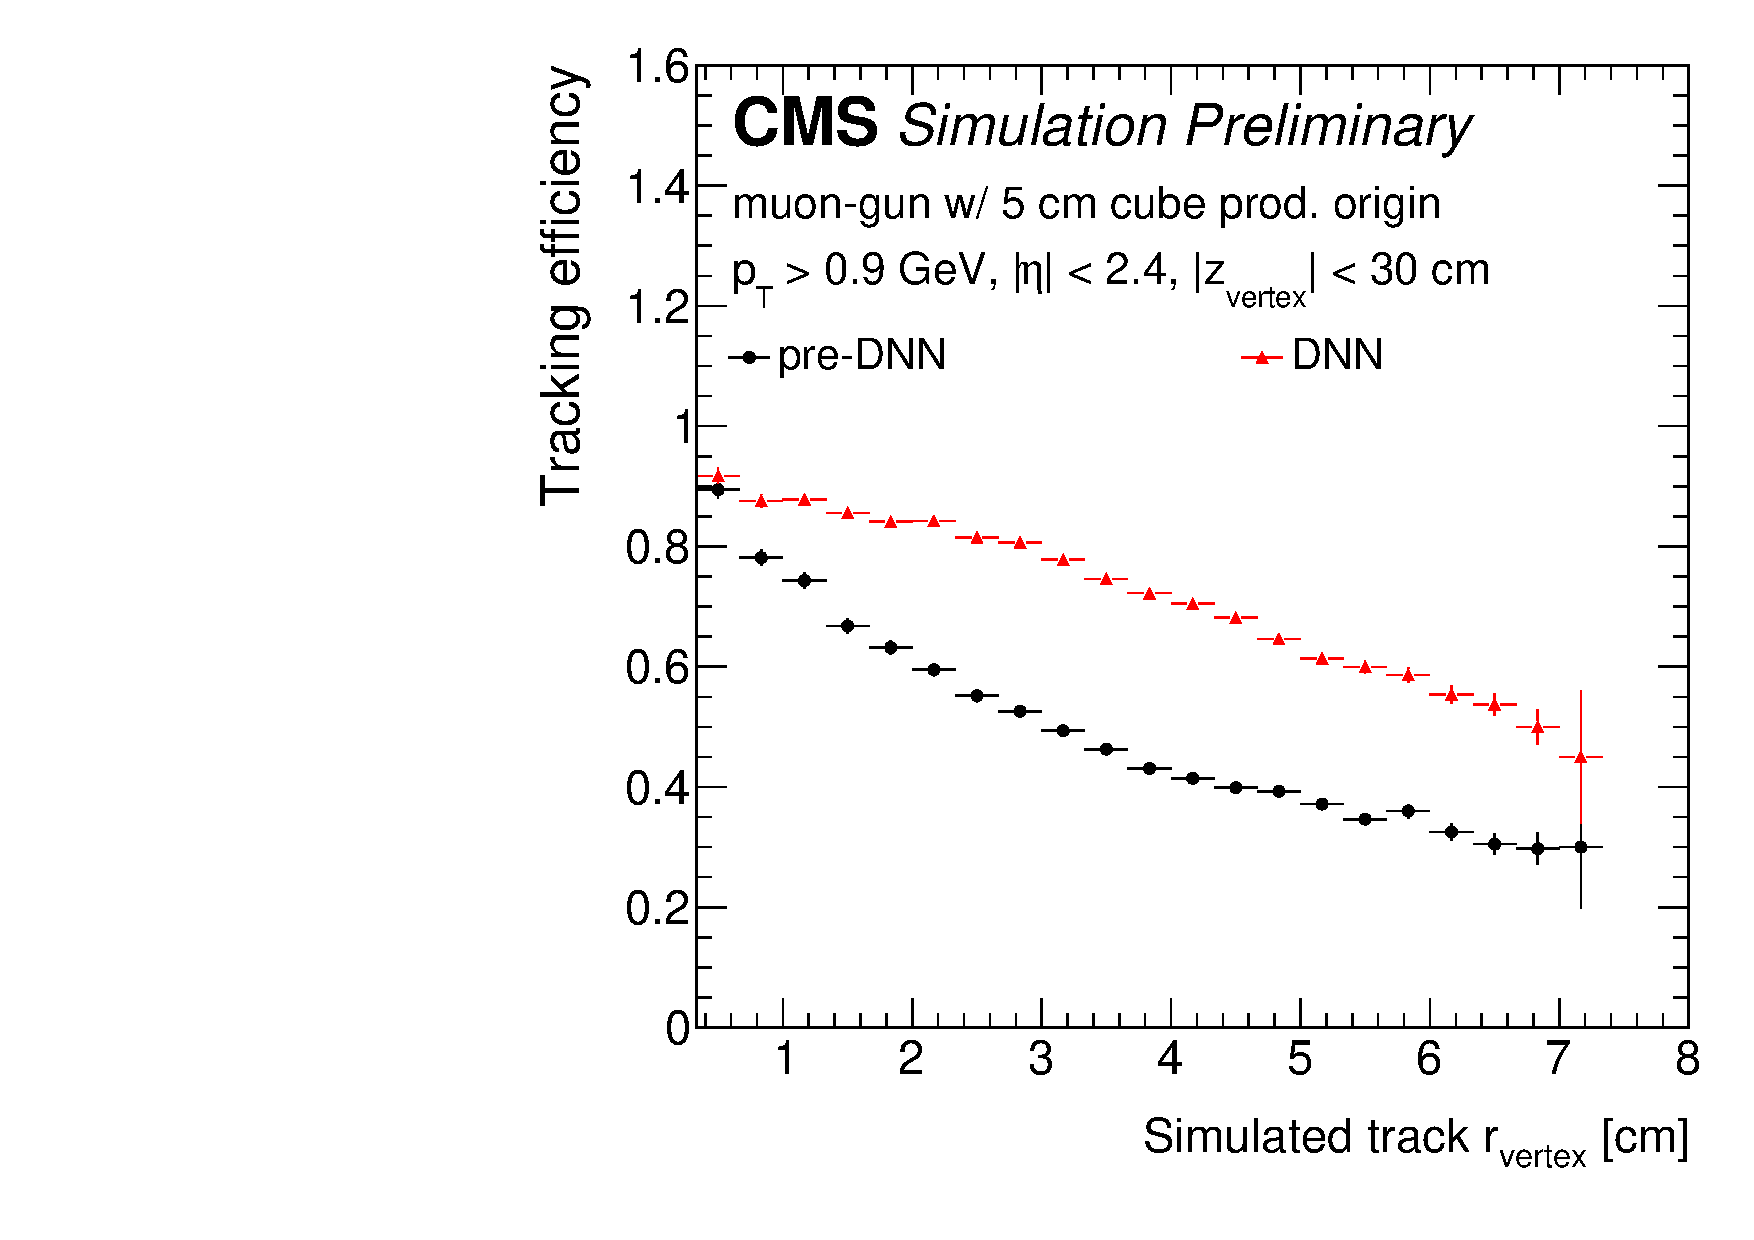
\includegraphics[width=0.45\linewidth]{fig/lst/standalone_DNNvsMaster_cube5_loweta_eff_vxy.pdf}\label{fig:t5dnn_eff_rvertex_cube}}
    \caption[LST efficiency for all TCs plotted as a function of $r_\text{vertex}$]{
        The LST efficiency for all TCs plotted as a function of $r_\text{vertex}$, i.e. the distance to the production vertex measured in the plane transverse to the beamline.
        This plot is made with 1000 \ttbar events with HL-LHC pile-up (left) and 10,000 ``muon-cube'' events where muons are produced at points uniformly distributed across a 5 cm cube (right).
        In both plots, it is clear that the T5-DNN recovers a significant amount of efficiency for displaced tracks.
        In the plot made for \ttbar events, there is a notable peak in the 18 to 20 cm $r_\text{vertex}$ bin.
        This spike in efficiency is due to the detector geometry: there is less detector material in that region, so contributions from material interactions there are lower than in neighboring bins.
    }
    \label{fig:t5dnn_dis}
\end{figure}

\begin{figure}[!htb]
    \centering
    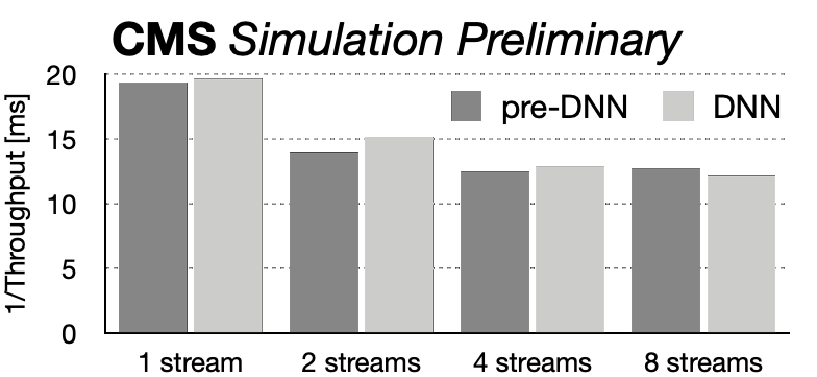
\includegraphics[width=0.75\linewidth]{fig/lst/throughput_vs_streams.pdf}
    \caption[LST throughput plotted for different numbers of parallel CUDA streams]{
        The LST throughput plotted for different numbers of parallel CUDA streams that are each opportunistically processing different events concurrently. 
        The throughput is measured before (dark grey) and after (light grey) the DNN is integrated into LST, showing no significant difference.
    }
    \label{fig:streams-vs-throughput}
\end{figure}

\section{Next steps}
Immediately, the success of the DNN begs the question, ``what is it doing so much better than what was done before?'' 
We are thus currently dissecting the DNN, determining which input features are most important and understanding how they are used to achieve the observed performance boost. 
At the same time, there are a number of additional opportunities for leveraging ML to improve LST. 
The same classification task can be improved for T3s, for instance, and duplicate removal---discerning between overlapping tracks---is a difficult, but vital step where efficiency is critical. 
Finally, more ambitious ML models could also be envisioned. 
Recent work suggests that graph neural networks (GNNs) could be used to do end-to-end track-finding and possibly track-fitting as well~\cite{Ju2021, DeZoortNature2023, lieret2023object}. 
We foresee these efforts integrated into LST, where LST provides a fast graph-building step---which is the slowest step in the current GNN tracking efforts---that feeds into a robust GNN-based tracking algorithm.

\section{Acknowledgements}
This chapter is a partial reproduction of the paper ``Improving tracking algorithms with machine learning: a case for line-segment tracking at the High Luminosity LHC'', in the proceedings of Connecting the Dots 2023 (arXiv:2403.13166). 
This work was supported by the U.S. National Science Foundation under Cooperative Agreements OAC-1836650, PHY-2323298, and PHY-2121686 and grant PHY-2209443.
